\documentclass[a4paper, 12pt, left=30mm, right=15mm, top=20mm, bottom=20mm]{report}
\usepackage[utf8]{inputenc}
\usepackage[russian]{babel}
\usepackage{mhchem} % for 13C
\usepackage{verbatim} % for multiline commentary 
\usepackage{graphicx} % for logo
\usepackage{titling} % for shift margins
\usepackage{blindtext} % for text-generation
\usepackage{setspace} % to set interval
\usepackage[numbers,sort&compress]{natbib} % for range cite [1-4]
\usepackage{todonotes} % todo

\newcommand{\CC}{C\nolinebreak\hspace{-.05em}\raisebox{.4ex}{\tiny\bf +}\nolinebreak\hspace{-.10em}\raisebox{.4ex}{\tiny\bf +}}
\def\CC{{C\nolinebreak[4]\hspace{-.05em}\raisebox{.4ex}{\tiny\bf ++}}} % define pretty C++

\graphicspath{ {./pics/} }
\begin{document}

\begin{titlepage}

	\begin{centering}
		
\includegraphics[width=0.25\textwidth]{logo.png}\par
	\end{centering}
	\centerline{Московский государственный университет имени М. В. Ломоносова}
	\centerline{Факультет вычислительной математики и кибернетики}
	\centerline{Кафедра математической кибернетики}
	\centerline{\hfill\hrulefill\hrulefill\hfill}
	\vfill
	\vfill
	\large
	\centerline{Стешин Семен Сергеевич}
	\vfill
	\Large
	\begin{centering}
		\textbf{Khnum: быстрая open-source программа \\ для расчета метаболических потоков \\ с использованием \ce{^{13}C}-углерода}
		
	\end{centering}
	\normalsize
	\vfill
	\centerline{Выпускная квалификационная работа}
	\vfill
	\vfill
	\begin{flushright}
	Научный руководитель:\\
	к.ф.м.н., доцент \\
	Шуплецов М. С.
	\end{flushright}
	\vfill
	\vfill
	\centerline{Москва --- 2020}

\end{titlepage}



\begin{abstract}
В биологии и медицине важно определять скорости метаболических потоков внутри клетки. 
Мощный метод решения этой задачи --- \ce{^{13}C}-Metabolic Flux Analysis --- анализ метаболических потоков с использованием  \ce{^{13}C}-углерода. 
В этом методе, исследователи проводят эксперимент и обрабатывают его результаты на компьютере. Для этого решают обратную задачу: подбирают такие параметры системы, чтобы результат компьютерной симуляции совпал с экспериментальными данными. Проблема в том, что современные программы для анализа метаболических потоков либо имеют закрытый код и платны для коммерческого использования, либо написаны неэффективно, из-за чего вычисления могут занимать недели для одного эксперимента. В этой работе проведен краткий обзор метода, его математических моделей, его программных реализаций, написана эффективная открытая программа для решения задачи на языке \CC{} и проведено сравнение с существующими аналогами.
\end{abstract}

\tableofcontents

\chapter{Введение}
\section{Мотивация}
Рак --- вторая по частоте причина смерти в мире\cite{Cancer_statistics}. Сто лет назад Отто Варбург заметил\cite{Warburg_effect} особенность раковых клеток: они склонны производить энергию с помощью активного гликолиза, вместо более эффективного окислительного фосфорилирования. Знание этого позволило находить опухоли с помощью позитронно-эмиссионной томографии, а Варбурга наградили Нобелевской премией.

Диабетом болеет 8.8\% людей в мире\cite{Diabetes_statistics}. Почти 4 миллиона в год умирает из-за этой болезни. Лечения пока нет, но есть симптоматическая терапия инъекциями инсулина. Раньше его получали из поджелудочных желез свиней и коров, но препарат было сложно очистить, поэтому иногда случались аллергические реакции. Все изменилось в 1978 году, когда компания Genentech смогла создать генетически-модифицированную кишечную палочку, которая в ходе жизнедеятельности производила чистый человеческий инсулин\cite{Genentech_paper}. Сейчас таким образом производят почти весь препарат.

В случае с эффектом Варбурга, открытие заключалось в изменении скорости химической реакции, протекающей внутри клетки. В случае с инсулином, решается задача метаболической инженерии --- увеличить скорость синтеза инсулина, не убив кишечную палочку. В обоих случаях надо уметь измерять скорости внутриклеточных химических реакций -- их называют потоками. Один из современных методов измерения потоков -- \emph{\ce{^{13}C}-Metabolic Flux Analysis} (далее \emph{MFA}), что переводится как анализ метаболических потоков. Его применяют в исследованиях рака\cite{Application_cancer_2009, Application_cancer_2012, Application_cancer_2013, Application_cancer_2015, Application_cancer_2017, Application_cancer_2018, Application_cancer_2018_2}, в~метаболической инженерии\cite{Application_engeneering_2009, Application_engeneering_2015, Application_engeneering_2017} и в других областях\cite{Application_other_2011, Application_other_2013, Application_other_2014}. Этому методу посвящена наша работа.

\section{\ce{^{13}C}-Metabolic Flux Analysis}
Введем основные понятия. Химические реакции, протекающие внутри клетки называют \emph{метаболическими потоками}, а их реагенты --- \emph{метаболитами}. Задача состоит в определении скоростей внутриклеточных потоков. 

Напрямую можно измерить только внешние потоки --- например, с какой скоростью поглощается глюкоза или с какой скоростью выделяется \ce{CO_2}. Внутриклеточные потоки восстанавливают из <<сцепленной>> информации, полученной в эксперименте. В методе \ce{^{13}C}-MFA для этого  используется субстрат, у которого некоторые атомы углерода заменены на стабильный тяжелый изотоп \ce{^{13}C}, называемый \emph{трейсером}\todo{проверить доступность субстратов углерода}
\footnote{На самом деле, использовать углерод не обязательно. В последнее время появились работы, использующие \ce{^{15}N} азот \cite{nitrogen_mfa} или \ce{^{34}S} серу \cite{sulfur_mfa}. Эти стабильные изотопы позволяют исследовать метаболические пути, в которых нет углерода, однако, для большинства приложений хватает более доступных субстратов с меченным углеродом.}. 
Этот субстрат скармливается колонии клеток, и тяжелый углерод распространяется по метаболитам в ходе химических реакций. То, как он распределится, зависит от скоростей потоков, поэтому узнав распределение, можно математическими методами восстановить значения метаболических потоков.

\subsection{Эксперимент}
Хотя, текущая работа концентрируется на численном моделировании, опишем эксперимент\cite[стр. 312]{protocol}. Исследователь выращивает клетки на субстрате, содержащем \ce{^{13}C}-углерод (обычно это глюкоза). Когда трейсер распределится по биологической системе, изолируем некоторые метаболиты: например, аминокислоты, полученные гидролизацией белков. Эти метаболиты содержат разное количество меченных атомов и, поэтому отличаются по массе. Найдем долю молекул разной тяжести. <<Взвешивать>> молекулы можно с помощью газовой хроматографии, при этом для каждого метаболита на выходе получим так называемый \emph{Mass Isotopomer Distribution} (далее \emph{MID}) --- вектор $M\!I\!D = [M_0, M_1, \ldots, M_n]$, где $M_i$ --- массовая доля метаболитов с $i$ атомами трейсера и $\sum_{i = 0}^{n} = 1$. Набор таких векторов станет входом для математической задачи. Подробные протоколы эксперимента можно найти в \cite{protocol_animal} для животных клеток и в \cite{protocol_plant} для растений.

\subsection{Математическая модель}
Существуют разные подходы к вычислению метаболических потоков. Чаще всего задачу решают как обратную. Для этого создают математическую модель, описывающую распределение трейсера в биологической системе при заданных скоростях потока; пишут программу для симуляции, а затем решают задачу регрессии: подбирают такие значения потоков, при которых распределение трейсера в симуляции совпадает с распределением, полученным в эксперименте.

Первым формальную модель прямой симуляции составил 	
Wolfgang Wiechert\cite{Wiechert_1997_1, Wiechert_1997_2} в 1997 году. Она использовала понятие изотопомера --- это молекулы одного вещества, имеющие одинаковое количество атомов изотопов, вообще говоря в разных позициях. За два года автор разработал математически эквивалентную модель кумомеров\cite{Wiechert_1999_3, Wiechert_1999_4}, которая быстрей расчитывалась на компьютере. В 2007 году Maciek R. Antoniewicz создал EMU-модель\cite{EMU_2007}, которая остается самой популярной среди программных реализаций. Так же существуют прямые модели\cite{Direct_MFA}, вероятностные модели на основе Марковских цепей\cite{Markov_chain_MFA} и другие\cite{Fluxomer_MFA}. В этой работе подробно разбирается EMU-модель.

\subsection{Компьютерные программы}

\chapter{Основные понятия}
\section{Глоссарий}
Приведем определения терминов 

\emph{\ce{^{13}C}-Metabolic Flux Analysis} --- Анализ метаболических потоков с использованием \ce{^{13}C}-углерода.

\emph{Метаболический поток} --- Внутриклеточная химическая реакция.

\emph{Метаболит} --- Реагент метаболического потока.
\clearpage

\section{Допущения}
Математическая модель для MFA основывается на нескольких допущениях о биологической системе\cite{Wiechert_1997_1}:
\begin{enumerate}
	\item Состояние системы можно представить в виде конечного множества однородных пулов. Каждому атому углерода внутриклеточного метаболита соответствует свой пул.
	\todo{Пулы?}
	
	\item Наблюдаемая система должна находится в стационарном состоянии. Для этого экспериментаторы выжидают некоторое время, пока трейсер распространяется по системе.\footnote{В этой работе рассматривается только \emph{Stationary MFA}, но существуют так же Non-Steady MFA\cite{NMFA}, в котором в клеточной культуре делают несколько замеров, пока трейсер распределяется, и Dynamic MFA\cite{DMFA}, в котором сами метаболические потоки меняются со временем. Эти модели не так развиты из-за своей вычислительной сложности.}
	
	\item Метаболическая карта должна быть полной. То есть для интересующих метаболических потоков должны быть известны все предшествующие химические реакции, и в них должна быть известна судьба каждого атома углерода.
	\todo{Дописать после неформального введения}
	
	\item Изотопические массовые эффекты несущественны. То есть химические реакции протекают одинаково как с \ce{^{12}C}, так и с \ce{^{13}C}. Это обычно верно, но массовые эффекты можно наблюдать в случае малых молекул типа \ce{CO_2}.
\end{enumerate}

Заметим, что разным математическим моделям могут соответствовать разные допущения. Этот вопрос подробно разбирался в работе \cite{formalizm_2017}, там же формально был доказан изоморфизм нескольких популярных моделей.
\clearpage

\section{Прямая симуляция}
Опишем модель распространения трейсера EMU, предложенную Мачеком Антониевичем в 2007 году\cite{EMU_2007}.

Пусть $A$ --- молекула. Любое непустое подмножество атомов углерода молекулы $A$ будем называть \emph{Elementary Metabolic Unit} (далее \emph{EMU}). Например, если $A$ состоит из трех атомов углерода, обозначим через $A_{13}$ EMU состоящий из первого и третьего атома углерода (на атомах углерода одной молекулы существует естественный порядок).

Будем рассматривать EMU-реакции. Всего можно выделить три типа: реакции конденсации(condensation), расщепления(cleavage) и унимолекулярная реакция(unimolecular). Для каждой реакции мы хотим понять, какое минимальное количество информации требуется, чтобы рассчитать MID продукта. Для всех реакций достаточно знать MID исходных веществ и тогда MID продукта рассчитывается по формалам с \ref{emu_reactions}.

\begin{figure}[t]
	\centering
	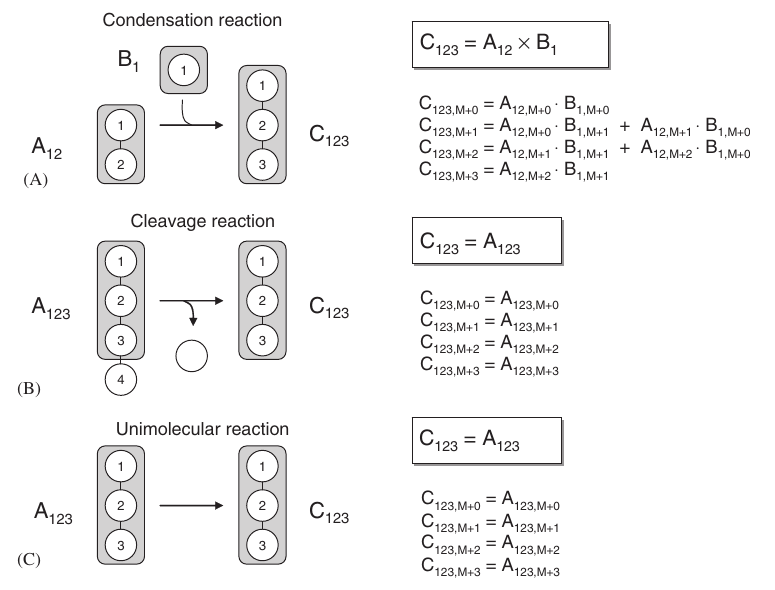
\includegraphics[width=1\textwidth]{emu_fig_1.png}
	\caption{EMU-реакции. Источник\cite{EMU_2007}}
	\label{emu_reactions}
\end{figure}

\section{Обратная задача}
Метод оптимизации.

\chapter{Постановка задачи}
\begin{itemize}
	\item Написать программу для расчета \ce{^{13}C}-MFA на языке \CC.
	\item Провести тестирование, сравнить скорость работы с существующими аналогами.
\end{itemize}

\chapter{Основная часть}
\section{Khnum}
Программа написана так-то. В ней то-то. 

\section{Тестирование}
Так убедился в корректности.

\section{Бенчмаркинг}
Во как быстро.

\chapter{Полученные результаты}
Кратко: написано, протестировано, замерено.

\section{Дальнейшая работа}
Че можно сделать


\begin{thebibliography}{XXXX}
	\bibitem{Cancer_statistics}
	Всемирная Ассоциация Здравоохранения. Cancer [Электронный ресурс] URL: https://www.who.int/news-room/fact-sheets/detail/cancer (дата обращения: 12.03.2020)
	
	\bibitem{Warburg_effect}
	Warburg O., Wind F., Negelein E. The metabolism of tumors in the body //The Journal of general physiology.--- 1927. --- Т. 8. --- №. 6. --- С. 519.
	
	\bibitem{Diabetes_statistics}
	Zimmet P. et al. Diabetes mellitus statistics on prevalence and mortality: facts and fallacies //Nature Reviews Endocrinology. --- 2016. --- Т. 12. --- №. 10. --- С. 616.
	
	\bibitem{Genentech_paper}
	Cohen S. N. et al. Construction of biologically functional bacterial plasmids in vitro //Proceedings of the National Academy of Sciences. --- 1973. --- Т. 70. --- №. 11. --- С. 3240--3244.
	
	\bibitem{Application_cancer_2009}
	Metallo C. M., Walther J. L., Stephanopoulos G. Evaluation of 13C isotopic tracers for metabolic flux analysis in mammalian cells //Journal of biotechnology. --- 2009. --- Т. 144. --- №. 3. --- С. 167--174.
	
	\bibitem{Application_cancer_2012}
	Walther J. L. et al. Optimization of 13C isotopic tracers for metabolic flux analysis in mammalian cells //Metabolic engineering. --- 2012. --- Т. 14. --- №. 2. --- С. 162--171.
	
	\bibitem{Application_cancer_2013}
	Hiller K., Metallo C. M. Profiling metabolic networks to study cancer metabolism //Current opinion in biotechnology. --- 2013. --- Т. 24. --- №. 1. --- С. 60--68.
	
	\bibitem{Application_cancer_2015}
	Boroughs L. K., DeBerardinis R. J. Metabolic pathways promoting cancer cell survival and growth //Nature cell biology. --- 2015. --- Т. 17. --- №. 4. --- С. 351--359.
	
	\bibitem{Application_cancer_2017}
	Dong W., Keibler M. A., Stephanopoulos G. Review of metabolic pathways activated in cancer cells as determined through isotopic labeling and network analysis //Metabolic engineering. --- 2017. --- Т. 43. --- С. 113--124.
	
	\bibitem{Application_cancer_2018}
	Antoniewicz M. R. A guide to 13 C metabolic flux analysis for the cancer biologist //Experimental \& molecular medicine. --- 2018. --- Т. 50. --- №. 4. --- С. 1--13.
	
	\bibitem{Application_cancer_2018_2}
	Badur M. G., Metallo C. M. Reverse engineering the cancer metabolic network using flux analysis to understand drivers of human disease //Metabolic engineering. --- 2018. --- Т. 45. --- С. 95--108.
	
	\bibitem{Application_engeneering_2009}
	Nakahigashi K. et al. Systematic phenome analysis of Escherichia coli multiple‐knockout mutants reveals hidden reactions in central carbon metabolism //Molecular systems biology. --- 2009. --- Т. 5. --- №. 1.
	
	\bibitem{Application_engeneering_2015}
	Crown S. B., Long C. P., Antoniewicz M. R. Integrated 13C-metabolic flux analysis of 14 parallel labeling experiments in Escherichia coli //Metabolic engineering. --- 2015. --- Т. 28. --- С. 151--158.
	
	\bibitem{Application_engeneering_2017}
	Long C. P. et al. Enzyme I facilitates reverse flux from pyruvate to phosphoenolpyruvate in Escherichia coli //Nature communications. --- 2017. --- Т. 8. --- №. 1. --- С. 1--8.
	
	\bibitem{Application_other_2011}
	Wahrheit J., Nicolae A., Heinzle E. Eukaryotic metabolism: measuring compartment fluxes //Biotechnology journal. --- 2011. --- Т. 6. --- №. 9. --- С. 1071--1085.
	
	\bibitem{Application_other_2013}
	Metallo C. M., Vander Heiden M. G. Understanding metabolic regulation and its influence on cell physiology //Molecular cell. --- 2013. --- Т. 49. --- №. 3. --- С. 388--398.
	
	\bibitem{Application_other_2014}
	Dieuaide-Noubhani M., Alonso A. P. (ed.). Plant metabolic flux analysis: methods and protocols. --- Humana Press, 2014.
	
	\bibitem{nitrogen_mfa}
	Nilsson R., Jain M. Simultaneous tracing of carbon and nitrogen isotopes in human cells //Molecular BioSystems. --- 2016. --- Т. 12. --- №. 6. --- С. 1929--1937.
	
	\bibitem{sulfur_mfa}
	Krömer J. O. et al. Accumulation of homolanthionine and activation of a novel pathway for isoleucine biosynthesis in Corynebacterium glutamicum McbR deletion strains //Journal of bacteriology. --- 2006. --- Т. 188. --- №. 2. --- С. 609--618.
	
	\bibitem{protocol}
	Systems Metabolic Engineering. Methods and Protocols. // Под ред. Alper, Hal S. --- 1 изд. Humana Press, 2013. --- 474 с.
	
	\bibitem{protocol_animal}
	(ed.). Metabolic flux analysis: methods and protocols. // Под ред. Krömer J. O., Nielsen L. K., Blank L. M. --- 1 изд. Humana Press, 2014. --- 329 с.
	
	\bibitem{protocol_plant}
	Plant metabolic flux analysis: methods and protocols. // Под ред. Dieuaide-Noubhani M., Alonso A.P. --- 1 изд. Humana Press, 2014. --- 366 с.
	
	\bibitem{Wiechert_1997_1}
	Wiechert W., de Graaf A. A. Bidirectional reaction steps in metabolic networks: I. Modeling and simulation of carbon isotope labeling experiments //Biotechnology and bioengineering. --- 1997. --- Т. 55. --- №. 1. --- С. 101--117.
	
	\bibitem{Wiechert_1997_2}
	Wiechert W. et al. Bidirectional reaction steps in metabolic networks: II. Flux estimation and statistical analysis //Biotechnology and bioengineering. --- 1997. --- Т. 55. --- №. 1. --- С. 118--135.
	
	\bibitem{Wiechert_1999_3}
	Wiechert W. et al. Bidirectional reaction steps in metabolic networks: III. Explicit solution and analysis of isotopomer labeling systems //Biotechnology and bioengineering. --- 1999. --- Т. 66. --- №. 2. --- С. 69--85.
	
	\bibitem{Wiechert_1999_4}
	Möllney M. et al. Bidirectional reaction steps in metabolic networks: IV. Optimal design of isotopomer labeling experiments //Biotechnology and bioengineering. --- 1999. --- Т. 66. --- №. 2. --- С. 86---103.
	
	\bibitem{Direct_MFA}
	Rantanen A. et al. Algorithms for 13C metabolic flux analysis. --- 2006.
	
	\bibitem{Markov_chain_MFA}
	Huo Y., Ji P. Continuous-Time Markov Chain–Based Flux Analysis in Metabolism //Journal of Computational Biology. --- 2014. --- Т. 21. --- №. 9. --- С. 691-698.
	
	\bibitem{Fluxomer_MFA}
	Srour O., Young J. D., Eldar Y. C. Fluxomers: a new approach for 13 C metabolic flux analysis //BMC systems biology. --- 2011. --- Т. 5. --- №. 1. --- С. 129.
	
	\bibitem{NMFA}
	Wiechert W., Nöh K. Isotopically non-stationary metabolic flux analysis: complex yet highly informative //Current opinion in biotechnology. --- 2013. --- Т. 24. --- №. 6. --- С. 979--986.
	
	\bibitem{DMFA}
	Leighty R. W., Antoniewicz M. R. Dynamic metabolic flux analysis (DMFA): a framework for determining fluxes at metabolic non-steady state //Metabolic engineering. --- 2011. --- Т. 13. --- №. 6. --- С. 745--755.
	
	\bibitem{formalizm_2017}
	Borkum M. I. et al. Modeling framework for isotopic labeling of heteronuclear moieties //Journal of cheminformatics. --- 2017. --- Т. 9. --- №. 1. --- С. 1--11.
	
	\bibitem{EMU_2007}
	Antoniewicz M. R., Kelleher J. K., Stephanopoulos G. Elementary metabolite units (EMU): a novel framework for modeling isotopic distributions //Metabolic engineering. --- 2007 --- Т. 9. --- №. 1. --- С. 68--86.
	
\end{thebibliography}

\end{document}          
